\chapter{Pohled na modelové testování}

Po sestavení všech požadavků na testování výrobků a na samotnou testovací laboratoř byl navržen způsob implementace testování založeného na modelech. V první fázi nasazování tohoto způsobu testování na produkty společnosti Conel bude uvažováno pouze systémové testování všech testovaných zařizení. Modely budou vytvářeny na největší abstraktní míře a to na úrovni jednotlivých funkcí. Zjednodušeně popsáno má každé zařízení definováno svůj model, který nadefinuje správce testovacího zařízení. Každému modelu jsou přiřazeny vlastnosti zařízení a funkce, které by mělo modelované zařízení podporovat. Každá funkce obsahuje sadu spustitelných testovacích procedur, pomocí kterých je skutečné zařízení testováno. Na závěr celého testování se porovnává výsledek spouštěných procedur na skutečných zařízních s výsledkem testu funkce na modelu zařízení.

\begin{figure}[h]
  \centering
  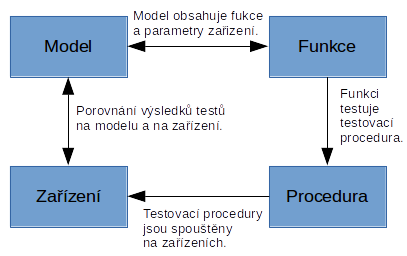
\includegraphics[width=.6\LW]{model_view}
  \caption{Pohled na modelové testování}
  \label{fig:model_view}
\end{figure}

\section{Funkce zařízení}

Základním pojmem tohoto přístupu bude funkce, kterou dané zařízení může podporovat. Každá funkcionalita jakéhokoliv testovaného zařízení je popsána právě touto základní vlastností. Příkladem takové funkce může být posílání sms zpráv. Každý router vlastnící bezdrátový modul umožňující tuto funkcionalitu bude tuto funkci poskytovat a naopak router bez bezdrátového modulu posílat sms zprávy zřejmně tuto funkcionalitu nebude podporovat.

Funkce definuje vlastnosti chování dané funkcionality zařízení, způsob testování a předpokládaný výsledek testu na modelu. Dále je možné definovat hiearchii funkcí, aby nebylo možné testovat nějakou funkci bez předchozího úspěšného testu jiné funkce. Například nemá smysl testovat nahrání nového firmwaru do výrobku pokud se nepovede úspěšně přeložit nový firmware.

\begin{figure}[h]
  \centering
  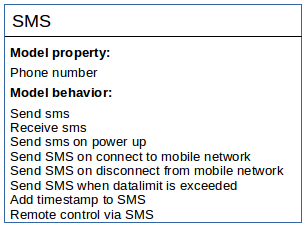
\includegraphics[width=.5\LW]{model_sms}
  \caption{Příklad funkce posílání sms zpráv}
  \label{fig:model_sms}
\end{figure}

\section{Testovací procedury}

Testování každé funkce bude prakticky realizováno testovacímy procedury. Každé funkci je přiřazena sada testovacích procedur, pomocí kterých jsou testovány všechny funkcionality dané funkce.

Testovací procedury jsou implementovány jako spustitelné BASHové skripty. Skripty jsou psány v jazyce BASH a pomocí testovacího API. Spuouštěnému skriptu se jako paramter předává identifikační číslo testovaného modelu a identifikační číslo testovaného releasu firmwaru. Skript spouští testy na daném routeru a porovnáná výsledky testů spuštěném na routeru s výsledky testů na modelu.

Prakticky připojení na konkrétní zařízení je realizováno pomocí telnet či ssh spojení. Tento princip nám umožňuje testovat jakékoliv zařízení umožňující komunikaci jedním z těchto protokolů. Dále je možné přidání dalších protokolů, ale u navrhované testovací aplikace si vystačím pouze s těmito protokoly.

\section{Model zařízení}

Každému výrobku je ve webovém rozhraní vytvořen model. Model obsahuje informace o daném výrobku jako je název testovaného výrobku, číslo portu do kterého je výrobek zapojen, IP adresu primárního portu výrobku a výchozí protokol komunikace se zařízením a další informace o tomto výrobku. Dále jsou tomuto modelu přiřazeny funkce, které daný model podporuje. Každý router má tedy k sobě přiřazen model obsahující informace o daném výrobku a množinu funkcí, jenž daný výrobek podporuje a mají být na něm testovány.

Při samotném testování výrobků testovací program testlab dle parametrů modelu  naváže s testovanými výrobky spojení. Po úspěšném navázaní spojení program spouští na daném zařízení testy definované v samotném modelu. Dále po provedení každého testu program porovnává výsledky testů spuštěných na testovaném zařízení s očekávanými výsledky testů spuštěných na modelu testovaného zařízení. Výsledky testů a případné chybové hlášky program zapisuje do databáze pro možnost vytvoření reportu z každého testování.

\section{Příklad modelu zařízení}

Pro snadnější pochopení implementace přístupu testování založené na modelech bude uveden příklad postupu vytváření modelu nového testovaného zařízení a jeho následné testování. Po ukončení základního vývoje je zařízení připojeno do testovací laboratoře. V dalším kroku je potřeba vytvořit model zařízení v testovací aplikaci. Model daného zařízení je vytvořen pomocí webové aplikace, jenž bude detailně popsána v kapitole věnující se webovému rozhraní testovací aplikace. Při vytváření modulu zařízení zadáme jeho parametry. Dále vytvořenému modelu přiřadíme funkce, které testované zařízení podporuje. Tímto krokem je ukončeno přidávání nového výrobku do automatického testování.

Pokud je model výrobku úspěšně přidán do testovacího zařízení, tak v dalším spuštění testování je nový výrobek již testován. Testovací program se připojí k testovanému zařízení a podle modelu spouští na testovaném zařízení jednotlivé testy a výsledky porovnává s výsledky testů provedených na modelu.

Konkrétním případem může být router LR77 v2F RS232, což je bezdrátový LTE router s volitelným sériovým rozhraním. Tomuto routeru přiřadíme IP adresu na primárním LAN interfacu 10.40.28.32, připojíme ho do třináctého portu switche. Výrobek podporuje komunikaci protokolem ssh i telnet a jako výchozí vybereme ssh protokol. Dále sou  routeru přiřazený následující funkce. SSH připojení a telnet připojení jsou funkce potřebné k připojení k routeru, pokud tedy testování těchto funkcí zkončí úspěšně pokračuje se na testování dalších funkcionalit routeru. Nyní je testován spojení do mobilní sítě ppp, jestliže je router úspěšně připojen je možné testovat Up/Down scripty routeru a zálohované připojení VRRP. Dále nezávisle na ppp spojení je testována funkcionalita sms zpráv a sériového rozhraní RS232.

\begin{figure}[h]
  \centering
  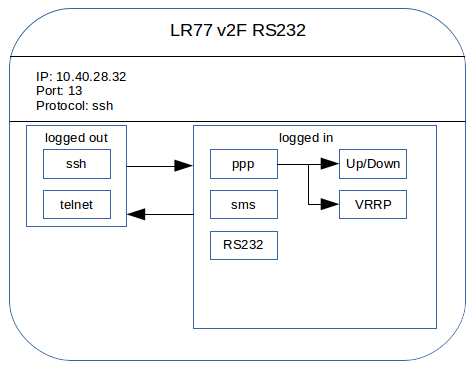
\includegraphics[width=.5\LW]{model_LR77}
  \caption{Příklad modelu routeru LR77 v2F RS232}
  \label{fig:model_LR77}
\end{figure}

\section{Výhody modelového přístupu}

Díky tomuto přístupu není potřeba při přidávání nového výrobku psát nové testovací skripty pro testování výrobku, ale pouze navolíme vlastnosti výrobku. Výrobek je testován dle testovacích procedur navolených funkcí. Pokud je vyvinuta nová funkcionalita jsou pro ní napsány testovací skripty a všem zařízením podporujícím tuto funkcionalitu se pouze přidá nová funkce v jejich modelu a není potřeba psát testovací procedury pro všechny možné routery. Pokud dojde ke změně zapojení v testovací laboratoři, opět není nutné přepisování všech testovacích skriptů routerů, kterých se tato změna týká, ale je pouze změněn model zařízení a testování funguje dále bez problémů.

\endinput
